% !TEX encoding = IsoLatin9

%%%%%%%%%%%%%%%%%%%%% SECTION 1
\section{L'algorithme minimax}

\begin{frame}
\frametitle{L'algorithme minimax}
\begin{itemize}
\setlength\itemsep{1em}
\item Algorithme issu de la th�orie des jeux
\item Il s'applique aux jeux � 2 joueurs, �  somme nulle
(1 gagnant/1perdant ou match nul) et � information compl�te.
\end{itemize}

\begin{block}{Principe}
Passer en revu un nombre limit� de coups
et les �valuer en fonction du b�n�fice pour le joueur
et sont adversaire
\end{block}

\end{frame}

\begin{frame}
\frametitle{Evaluation d'un position}
\begin{columns}
\column{0.7\textwidth}
\begin{figure}
\centering
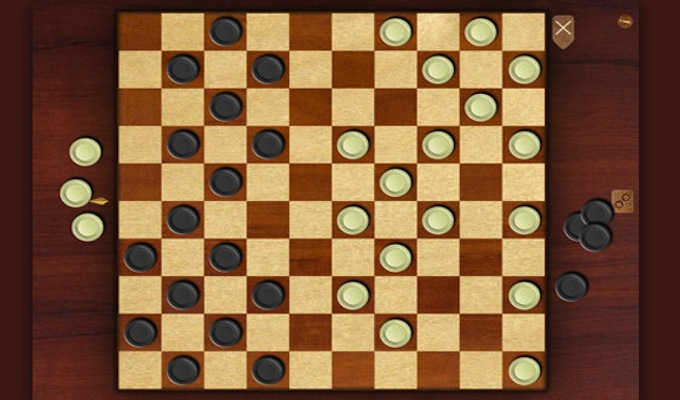
\includegraphics[width=8cm]{./fig/dames.jpg}
\end{figure}
\column{0.25\textwidth}
Joueur : Blancs\\
Adversaires : Noirs \\
\end{columns}
\vspace{1em}
Evaluation = Nbre de pions blancs - Nbre de pions noirs (ici = 1)
\end{frame}

\begin{frame}
\frametitle<1-8|handout:1-2>{Arbre minimax}
\frametitle<9-|handout:3>{Variante Negamax}
\begin{figure}
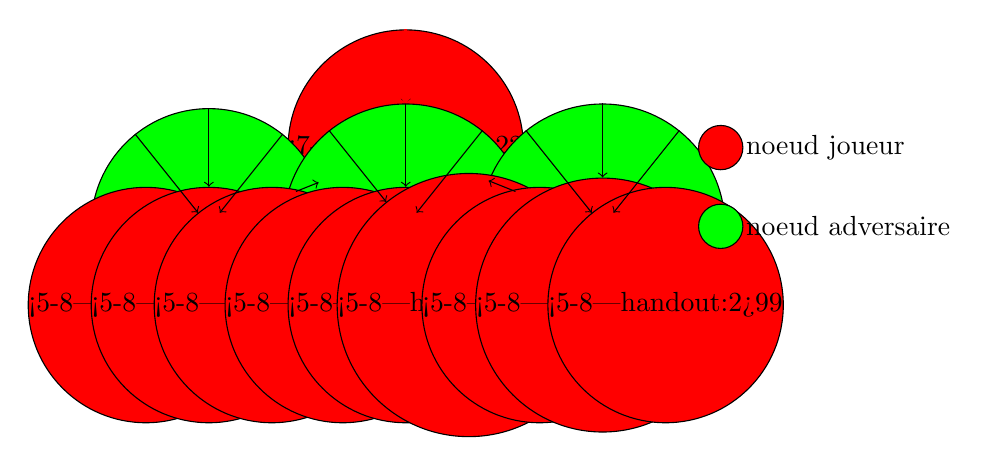
\begin{tikzpicture} [
  remember picture,
  auto,
  noeud/.style = {circle,draw=black,inner sep = 0pt, radius = 16pt,minimum size = 16pt},
  line/.style = {draw,->},
]

 \node [noeud, fill = red] (rac) {\temporal<7-8|handout:2>{}{2}{2} };

\visible<2->{ \node [noeud, fill = green, below of = rac, xshift = -2.5cm] (fg) {\temporal<6-8|handout:2>{}{0}{0} };}
\visible<2->{ \node [noeud, fill = green, below of = rac] (fm) {\temporal<6-8|handout:2>{}{2}{-2} };}
\visible<2->{ \node[noeud, fill = green, below of = rac, xshift = +2.5cm] (fd) {\temporal<6-8|handout:2>{}{-1}{1} };}

\visible<3->{ \node [noeud, fill = red, below of = fg, xshift = -0.8cm] (fgg) {\temporal<5-8|handout:2>{}{9}{9} };}
\visible<3->{ \node [noeud, fill = red,below of = fg] (fgm) {\temporal<5-8|handout:2>{}{7}{7} };}
\visible<3->{ \node [noeud, fill = red,below of = fg, xshift = 0.8cm] (fgd) {\temporal<5-8|handout:2>{}{0}{0} };}


\visible<3->{ \node [noeud, fill = red, below of = fm, xshift = -0.8cm] (fmg) {\temporal<5-8|handout:2>{}{2}{2} };}
\visible<3->{ \node [noeud, fill = red,below of = fm] (fmm) {\temporal<5-8|handout:2>{}{5}{5} };}
\visible<3->{ \node [noeud, fill = red,below of = fm, xshift = 0.8cm] (fmd) {\temporal<5-8|handout:2>{}{$\infty$}{$\infty$} };}


\visible<3->{ \node [noeud, fill = red, below of = fd, xshift = -0.8cm] (fdg) {\temporal<5-8|handout:2>{}{8}{8} };}
\visible<3->{ \node [noeud, fill = red,below of = fd] (fdm) {\temporal<5-8|handout:2>{}{-1}{-1} };}
\visible<3->{ \node [noeud, fill = red,below of = fd, xshift = 0.8cm] (fdd) {\temporal<5-8|handout:2>{}{9}{9} };}


\node [noeud, right of = rac, xshift = 3 cm,  fill = red] (ljoueur) {};
\node [noeud, below of = ljoueur, fill = green] (ladv) {};
\node [right of = ljoueur, anchor = west,xshift = -0.8cm] {noeud joueur};
\node [right of = ladv, anchor = west, xshift = -0.8cm] {noeud adversaire};

%\node [right of = fdd] {feuille};

 \begin{scope}[every path/.style=line]
\path<2-> (rac) -- (fg) ;
\path<2-> (rac) -- (fm) ;
\path<2-> (rac) -- (fd) ;

\path<3-> (fg) -- (fgg) ;
\path<3-> (fg) -- (fgm) ;
\path<3-> (fg) -- (fgd) ;


\path<3->  (fm) -- (fmg) ;
\path<3->  (fm) -- (fmm) ;
\path<3->  (fm) -- (fmd) ;


\path<3->  (fd) -- (fdg) ;
\path<3->  (fd) -- (fdm) ;
\path<3->  (fd) -- (fdd) ;

\end{scope}
\path <8-9|handout:2-3> [line, very thick, draw=red] (rac) -- (fm) ;
\end{tikzpicture}
\end{figure}

\begin{overlayarea}{\textwidth}{5cm}

\begin{onlyenv}<1-4|handout:1>
Position initiale donn�e\\
Question : quel coup jouer ?
\begin{enumerate}
\item<2-> On explore tous les coups possibles
\item<3-> Pour chaque coup, on explore les r�ponses possibles de l'adversaire
\item<4-> On continue jusqu'� une profondeur fix�e.
\end{enumerate}
\end{onlyenv}

\begin{onlyenv}<5-8|handout:2>
\begin{enumerate}
\item<5-> On �value les positions des noeuds terminaux (feuilles)
\item<6-> On �value les noeuds parents
\begin{itemize}
\item<6-> Si le noeud est  \textcolor{red}{joueur} : \texttt{eval(noeud) = max (fils)}
\item<6-> Si le noeud est \textcolor{green}{adversaire} : \texttt{eval(noeud) = min (fils)}
\end{itemize}
\item<7-> Lorsqu'on arrive � la racine, on choisit le coup qui am�ne au fils maximum
\end{enumerate}
\end{onlyenv}

\begin{onlyenv}<9|handout:3>
\begin{enumerate}
\item Evaluation des feuilles
 \begin{itemize}
\item Si le noeud est  \textcolor{red}{joueur} : \texttt{eval(feuille) = f()}
\item Si le noeud est \textcolor{green}{adversaire} : \texttt{eval(noeud) = -f()}
\end{itemize}
\item Evaluation des noeuds : \texttt{eval(noeud) = max (-eval(fils))}
\item Lorsqu'on arrive � la racine, on choisit le coup qui am�ne au fils maximum
\end{enumerate}
\begin{alertblock}{}
La fonction d'�valuation doit �tre sym�trique
\end{alertblock}
\end{onlyenv}

\end{overlayarea}

\end{frame}